\documentclass{article}
\setlength{\parskip}{5pt} % esp. entre parrafos
\setlength{\parindent}{0pt} % esp. al inicio de un parrafo
\usepackage{listings} % listings
\usepackage{color} %colores
\usepackage{amsmath} % mates
\usepackage[sort&compress,numbers]{natbib} % referencias
\usepackage{url} % que las URLs se vean lindos
\usepackage[top=15mm,left=25mm,right=25mm,bottom=20mm]{geometry} % margenes 
\usepackage{hyperref} % ligas de URLs
\usepackage{graphicx} % poner figuras
\usepackage[spanish]{babel} % otros idiomas
\usepackage{subfigure}


\author{Claudia Lizeth Hern\'andez Ram\'irez} % author
\title{Homework 7 - B\'usqueda local} % titulo
\date{\today}

\definecolor{myfucsia}{rgb}{1, 0.078, 0.576}
\definecolor{mygray}{rgb}{0.752, 0.752, 0.752}
\definecolor{mypurple}{rgb}{0.580, 0, 0.827}
\lstset{ 
  backgroundcolor=\color{mygray},
  commentstyle=\color{myfucsia},
  keywordstyle=\color{mypurple}, 
  numberstyle=\tiny\color{myfucsia}
  stringstyle=\color{mypurple}, 
  breaklines=true,
}


\begin{document} % inicia contenido

\maketitle % cabecera



% INTRODUCCIOOOOOOOOOOOON
\section{Introducci\'{o}n}\label{intro} % seccion y etiqueta
La tarea se trata de maximizar alg\'una variante de la funci\'on bidimensional ejemplo, \texttt{g(x,y)}, con restricciones tipo \texttt{-3$\leq$x,y$\leq$3}, con la misma t\'ecnica del ejemplo unidimensional. La posici\'on actual es un par \texttt{x,y} y se ocupan dos movimientos aleatorios, $\triangle$x y $\triangle$y, cuyas combinaciones posibles proveen ocho posiciones vecino, de los cuales aquella que logra el mayor valor para \texttt{g} es seleccionado. Dibujado en tres dimensiones, \texttt{g(x,y)}.


% DESARROLLOOOOOOOOOOOO
\section{Desarrollo}\label{desarrollo} % Desarrollo de la tarea
Comenc\'e trabajando con el c\'odigo base\citep{CBase} al cual se le realizaron varios cambios para lograr el objetivo de la tarea.Dentro de las modificaciones que se implementaron estan: cambiar la funci\'on y hacerla bidimensional con otros intervalos de trabajo, se agreg\'o un ciclo \texttt{FOR} para variar el paso con el que se mueven los puntos rojos y otro ciclo \texttt{FOR} para las repeticiones. \newline
La funci\'on con la que trabaje es:
\begin{equation}
f(x,y) = (x^2) -8 * x -10 * (5 * sin(x)) - (y^2) * (5* sin(y))
\label{funcion}
\end{equation}
Las restricciones de mi funci\'on son : -5$\leq$x, y$\leq$5.


\begin{figure}[h!]
\centering
\subfigure[Funci\'on graficada en 3D.]{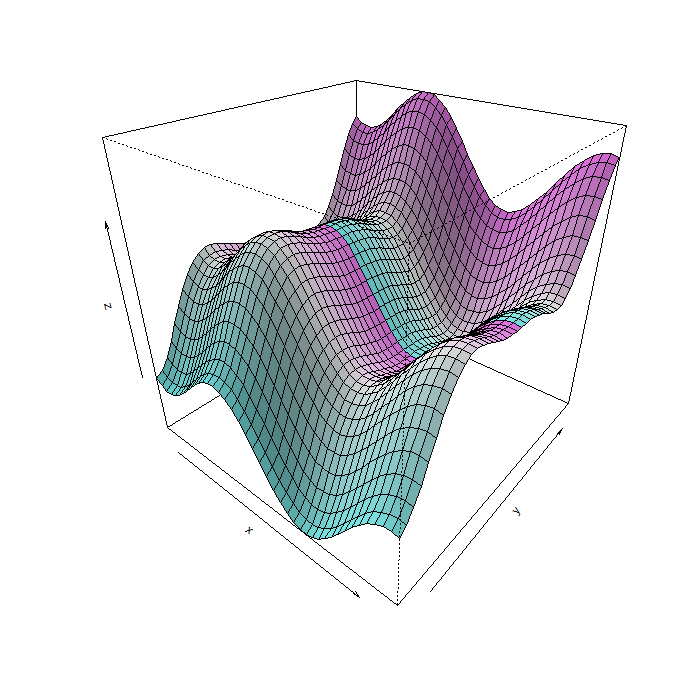
\includegraphics[width=60mm]{p7_3d2.png}}
\subfigure[Proyecci\'on del plano $xy$.]{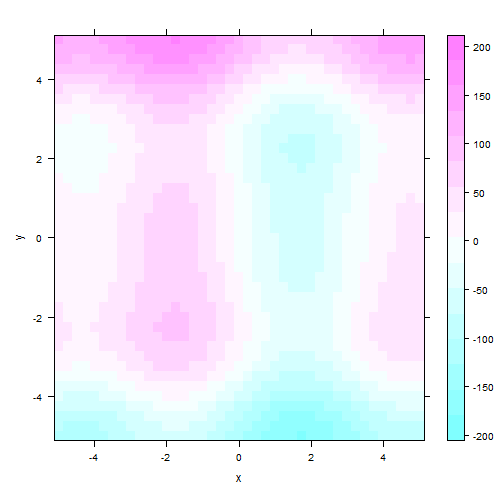
\includegraphics[width=60mm]{p7_flat_2.png}}
\caption{Visualizaci\'on gráfica de la funci\'on \eqref{funcion}.} 
\label{f1}
\end{figure}
\newpage

\begin{lstlisting}[language=R, caption= C\'odigo proyecci\'on del plano \texttt{xy}.]
g <- function(x,y) {
  return(((x^2) - 8 * x - 10 * (5 * sin(x)) - (y^2) * (5 * sin(y)) ))
}
x <- seq(-5, 5, 0.25) 
y <- x
z <- outer(x, y, g)
dimnames(z) = list(x, y)
library(reshape2)
d = melt(z)
names(d) = c("x", "y", "z")
library(lattice)
png("p7_flat_2.png", width = 500, height = 500)
levelplot(z ~ x * y, data = d, col.regions = cm.colors(100))
graphics.off()
\end{lstlisting}

\begin{lstlisting}[language=R, caption= C\'odigo gr\'afica 3D.]
g <- function(x, y) {
  return(((x^2) - 8 * x - 10 * (5 * sin(x)) - (y^2) * (5 * sin(y)) ))
}
x <- seq(-5, 5, 0.25)
y <-  x
z <- outer(x, y, g)
png("p7_3d.png", width=700, height=700)
persp(x, y, z, shade=0.2, col=cm.colors(800) , theta=40, phi=30)
graphics.off()
\end{lstlisting}

\begin{lstlisting}[language=R, caption= C\'odigo para obtener los puntos.]
datos<- data.frame()
g <- function(x,y) {
  return(((x^2) - 8 * x - 10 * (5 * sin(x)) - (y^2) * (5 * sin(y)) ))
}

x <- seq(-5, 5, 0.25) 
y <- x
z <- outer(x, y, g)

low <- -5
high <- 5
pasos <- seq(0.25, 4, 0.25) 
repe = 1:30
replicas <- 50 #Cuantos puntitos


for (step in pasos) {
  for (reply in repe){ #hacer repeticiones del experimento
    replica <- function(t) {
      curr <- c(runif(1, low, high), runif(1, low, high))
      best <- curr
      for (tiempo in 1:t) {
      [...]
\end{lstlisting}

\newpage El c\'odigo completo se encuentra en mi repositorio\citep{Ccompleto} .

En base a otro c\'odigo visto en clase\citep{Cimagenes} gener\'e las im\'agenes para mi gif\citep{Gif}.

Almacen\'e la informaci\'on generada con mi c\'odigo en un data frame, de donde posteriormente extraje los datos para generar mi \texttt{boxplot} y realizar pruebas estad\'isticas.

\begin{lstlisting}[language=R, caption= C\'odigo Boxplot.]
datos$Paso = as.factor(datos$Paso)
ggplot(datos, aes(x= Paso, y= Minimo, fill= Paso, )) + 
  geom_boxplot(fill = cm.colors(16))+
  labs(x = "Paso", y = "Valor minimo")
\end{lstlisting}



\begin{lstlisting}[language=R, caption= C\'odigo pruebas estad\'isticas.]
#Estadisitica - 
#con p menor a 0.05 se rechaza hipotesis nula H0
#H0: los datos proceden de una distribucion normal
#H1: los datos no proceden de una distribucion normal
tapply(datos$Minimo, datos$Paso, shapiro.test) #Shapiro

datos%>% #Datos individuales
  group_by(Paso) %>%
  summarise(
    
    promedio = mean(Minimo, na.rm = TRUE),
    desviacion_std = sd(Minimo, na.rm = TRUE),
    varianza = sd(Minimo, na.rm = TRUE)^2,
    mediana = median(Minimo, na.rm = TRUE),
    rango_intercuartil = IQR(Minimo, na.rm = TRUE)
  )

kruskal.test(Minimo ~ Paso, data = datos) #Kruskal
pairwise.wilcox.test(datos$Minimo, datos$Paso) #Wilcox
\end{lstlisting}



\begin{figure}[htbp]
\centering
\subfigure[Paso 1.]
{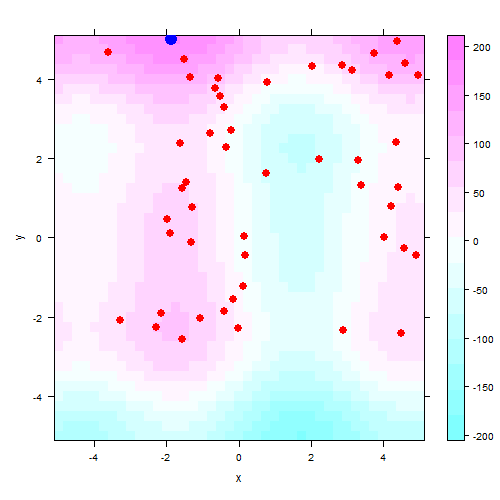
\includegraphics[width=50mm]{t7_1.png}}
\subfigure[Paso 6.]
{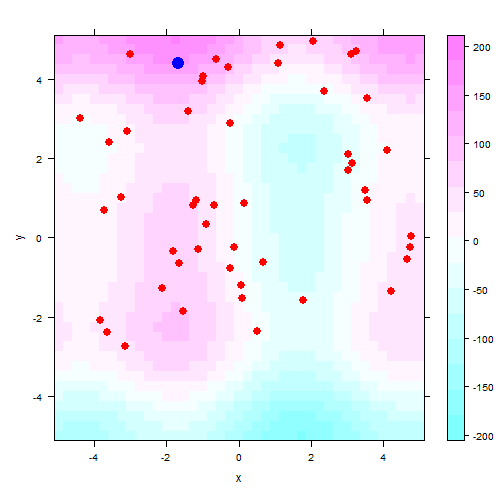
\includegraphics[width=50mm]{t7_6.png}}
\subfigure[Paso 11.]
{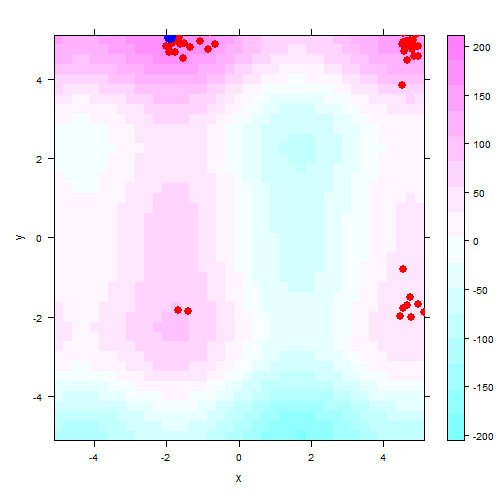
\includegraphics[width=50mm]{t7_11.png}}
\subfigure[Paso 16.]
{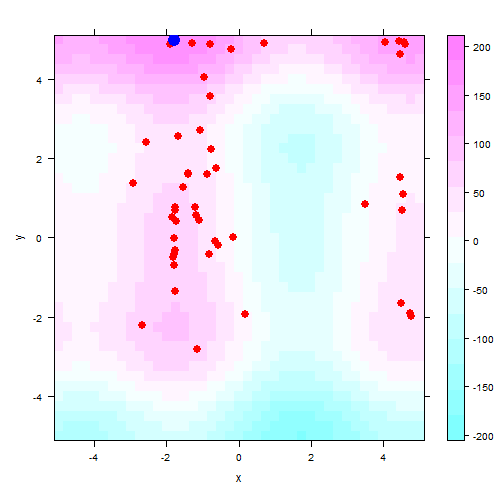
\includegraphics[width=50mm]{t7_16.png}}
\subfigure[Paso 21.]
{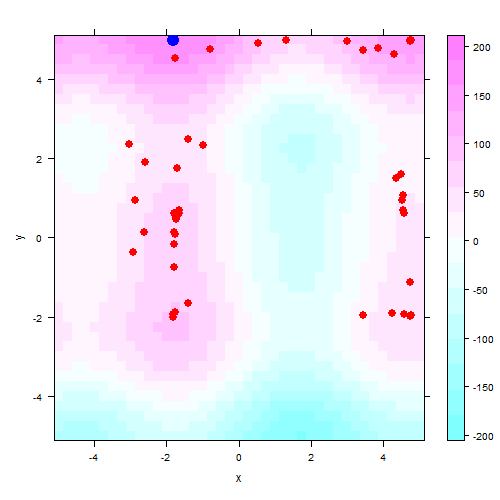
\includegraphics[width=50mm]{t7_21.png}}
\subfigure[Paso 26.]
{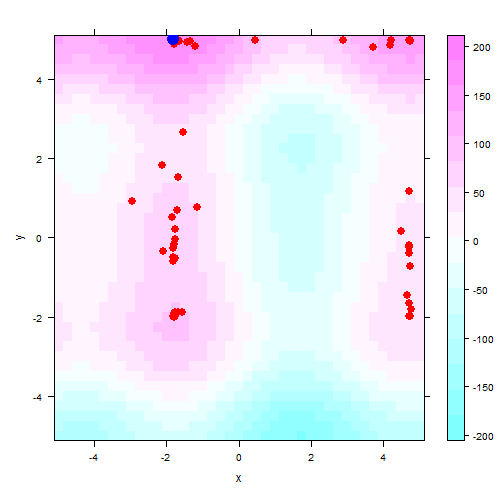
\includegraphics[width=50mm]{t7_26.png}}
\subfigure[Paso 31.]
{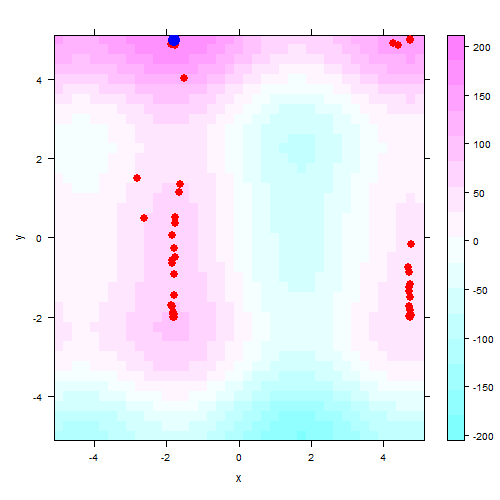
\includegraphics[width=50mm]{t7_31.png}}
\subfigure[Paso 36.]
{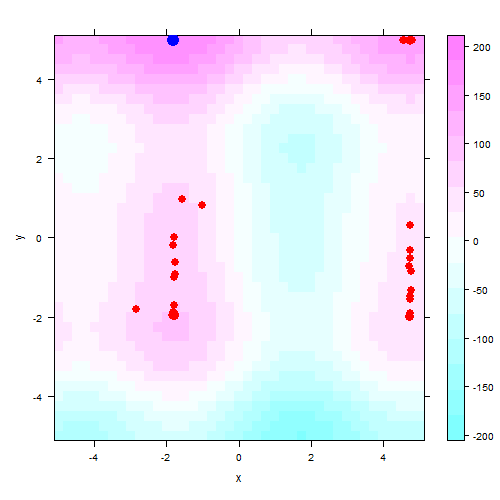
\includegraphics[width=50mm]{t7_36.png}}
\subfigure[Paso 40.]
{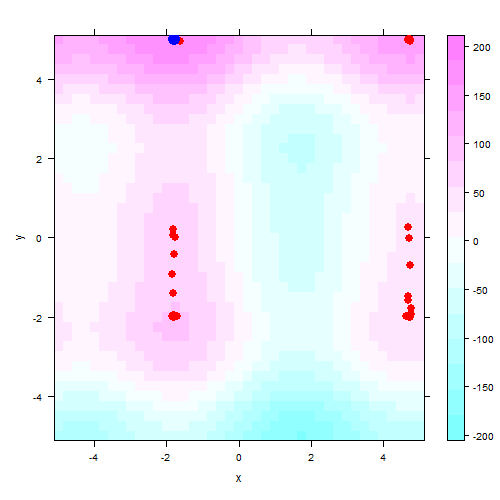
\includegraphics[width=50mm]{t7_40.png}}
\caption{Busqueda local de la funci\'on \eqref{funcion} a p =0.25.} 
\label{f2}
\end{figure}

\begin{figure}[htbp]
\centering
\subfigure[Paso 1.]
{\includegraphics[width=50mm]{3t7_1.png}}
\subfigure[Paso 6.]
{\includegraphics[width=50mm]{3t7_6.png}}
\subfigure[Paso 11.]
{\includegraphics[width=50mm]{3t7_11.png}}
\subfigure[Paso 16.]
{\includegraphics[width=50mm]{3t7_16.png}}
\subfigure[Paso 21.]
{\includegraphics[width=50mm]{3t7_21.png}}
\subfigure[Paso 26.]
{\includegraphics[width=50mm]{3t7_26.png}}
\subfigure[Paso 31.]
{\includegraphics[width=50mm]{3t7_31.png}}
\subfigure[Paso 36.]
{\includegraphics[width=50mm]{3t7_36.png}}
\subfigure[Paso 40.]
{\includegraphics[width=50mm]{3t7_40.png}}
\caption{Busqueda local de la funci\'on \eqref{funcion} a p =3.50.} 
\label{f3}
\end{figure}


\newpage
\section{Estad\'istica}

\begin{figure}[htbp] % figura
    \centering
    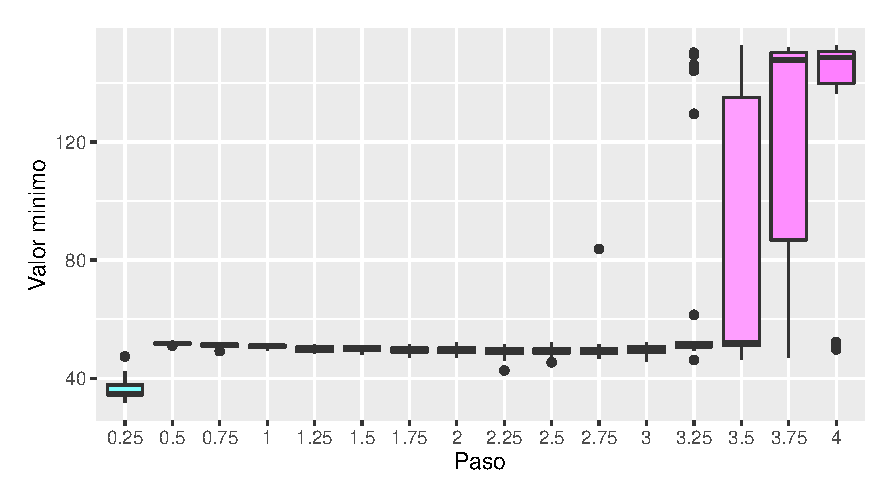
\includegraphics[width=120mm]{Rplot02.eps} % archivo
    \caption{Valor m\'inimo de puntos rojos por paso.}
    \label{Figura 3}
\end{figure}

\begin{table}[ht]
    \centering
    \caption{Resultados obtenidos de prueba de normalidad de Shapiro.} 
    \begin{tabular}{|r|r|r|r|}
    \hline
    Combinaci\'on & W value & P value & ¿Se acepta H0?  \\
    \hline
    0.25 & 0.8080 & $9.2\times 10^{-05}$ & no \\
    \hline 
    0.50 & 0.9389 & 0.0851 & s\'i  \\
    \hline 
    0.75 & 0.8864 & 0.0039 & no \\
    \hline
    1.00 & 0.9672 & 0.4668 & s\'i \\
    \hline
    1.25 & 0.9248 & 0.0359 & no \\
    \hline
    1.50 & 0.9761 & 0.7159 & s\'i \\
    \hline
    1.75 & 0.9722 & 0.6035 & s\'i \\
    \hline
    2.00 & 0.9835 & 0.9089 & s\'i \\
    \hline
    2.25 & 0.8756 & 0.0022 & no \\
    \hline
    2.50 & 0.9339 & 0.0627 & s\'i \\
    \hline
    2.75 & 0.3460 & $1.7\times 10^{-10}$ & no \\
    \hline
    3.00 & 0.9448 & 0.1227 & s\'i \\
    \hline
    3.25 & 0.5086 & $6.6\times 10^{-09}$ & no \\
    \hline
    3.50 & 0.6749 & $6.8\times 10^{-07}$ & no \\
    \hline
    3.75 & 0.6306 & $1.7\times 10^{-07}$ & no \\
    \hline
    4.00 & 0.5631 & $2.6\times 10^{-08}$ & no \\
    \hline
\end{tabular}
    \label{cuadro 1}
\end{table}
\newpage 


\begin{table}[htbp]
    \centering
    \caption{Informaci\'on individual de los datos.} 
    \begin{tabular}{|r|r|r|r|r|r|r|}
    \hline
    Carga & Participantes & Promedio & Desv. Std. & Varianza & Mediana & Rango Intercuartil  \\
    \hline
    0.25 & 30 & 36.50 & 3.52 & 12.40 & 34.70 & 3.22 \\
    \hline
    0.50 & 30 & 51.70 & 0.25 & 0.06 & 51.80 & 0.31 \\
    \hline
    0.75 & 30 & 51.10 & 0.59 & 0.35 & 51.20 & 0.78 \\
    \hline
    1.00 & 30 & 50.80 & 0.54 & 0.29 & 50.90 & 0.78 \\
    \hline
    1.25 & 30 & 50.00 & 0.86 & 0.75 & 50.20 & 1.56 \\
    \hline
    1.50 & 30 & 49.90 & 0.75 & 0.56 & 50.00 & 1.21 \\
    \hline
    1.75 & 30 & 49.40 & 1.07 & 1.15 & 49.60 & 1.36 \\
    \hline
    2.00 & 30 & 49.40 & 1.24 & 1.54 & 49.50 & 1.64 \\
    \hline
    2.25 & 30 & 49.00 & 1.80 & 3.26 & 49.30 & 1.86 \\
    \hline
    2.50 & 30 & 49.10 & 1.37 & 1.88 & 49.30 & 1.41 \\
    \hline
    2.75 & 30 & 50.30 & 6.46 & 41.70 & 49.30 & 1.52 \\
    \hline
    3.00 & 30 & 49.60 & 1.72 & 2.95 & 50.10 & 2.18 \\
    \hline
    3.25 & 30 & 66.70 & 35.30 & 1248 & 51.30 & 1.57 \\
    \hline
    3.50 & 30 & 82.60 & 45.10 & 2031 & 52.00 & 84.00 \\
    \hline
    3.75 & 30 & 123.0 & 42.60 & 1812 & 148.0 & 63.40 \\
    \hline
    4.00 & 30 & 129.0 & 39.80 & 1583 & 148.0 & 10.80 \\
    \hline
\end{tabular}
    \label{cuadro 2}
\end{table}



\begin{table}[htbp]
    \centering
    \caption{Resultados obtenidos de prueba Kruskal-Wallis.} 
    \begin{tabular}{|r|r|r|}
    \hline
    Chi cuadrada & DF & P  \\
    \hline
    308.88 & 15 & $2.2\times 10^{-16}$ \\
    \hline
\end{tabular}
    \label{cuadro 3}
\end{table}



\begin{table}[htb]
    \centering
    \caption{Diferencias entre grupos.} 
    \begin{tabular}{|r|r|r|r|r|r|r|r|r|}
    \hline
    "" & 0.25 & 0.50 & 0.75 & 1.00 & 1.25 & 1.50 & 1.75 & 2.00 \\
    \hline
    0.50 & $2.0\times 10^{-15}$ &  &  &  &  &  &  & \\
    \hline
    0.75 & $2.0\times 10^{-15}$ & $3.3\times 10^{-06}$ &  &  &  &  &  & \\
    \hline
    1.00 & $2.0\times 10^{-15}$ & $6.7\times 10^{-11}$ & 0.51 &  &  &  &  &  \\
    \hline
    1.25 & $2.0\times 10^{-15}$ & $2.1\times 10^{-14}$ & $2.6\times 10^{-05}$ & 0.02 &  &  &  &  \\
    \hline
    1.50 & $2.0\times 10^{-15}$ & $7.5\times 10^{-15}$ & $9.7\times 10^{-07}$ & $5.4\times 10^{-04}$ & 1.00 &  &  &  \\
    \hline
    1.75 & $3.9\times 10^{-15}$ & $7.5\times 10^{-15}$ & $2.8\times 10^{-08}$ & $4.9\times 10^{-06}$ & 1.00 & 1.00 &  &  \\
    \hline
    2.00 & $7.5\times 10^{-15}$ & $6.7\times 10^{-11}$ & $1.2\times 10^{-06}$ & $7.2\times 10^{-05}$ & 1.00 & 1.00 & 1.00 &  \\
    \hline
    2.25 & $3.3\times 10^{-14}$ & $1.3\times 10^{-14}$ & $1.2\times 10^{-07}$ & $3.1\times 10^{-05}$ & 0.64 & 1.00 & 1.00 & 1.00 \\
    \hline
    2.50 & $1.3\times 10^{-14}$ & $3.1\times 10^{-11}$ & $5.4\times 10^{-09}$ & $4.2\times 10^{-07}$ & 0.26 & 0.26 & 1.00 & 1.00 \\
    \hline
    2.75 & $2.1\times 10^{-14}$ & $5.5\times 10^{-11}$ & $2.0\times 10^{-07}$ & $6.5\times 10^{-06}$ & 0.32 & 1.00 & 1.00 & 1.00 \\
    \hline
    3.00 & $2.1\times 10^{-14}$ & $4.2\times 10^{-08}$ & $7.3\times 10^{-03}$ & 0.36 & 1.00 & 1.00 & 1.00 & 1.00 \\
    \hline
    3.25 & $3.9\times 10^{-15}$ & 1.00 & 1.00 & 0.61 & $4\times 10^{-04}$ & $1.4\times 10^{-04}$ & $7.9\times 10^{-06}$ & $3.3\times 10^{-05}$ \\
    \hline
    3.50 & $7.5\times 10^{-15}$ & 1.00 & 0.25 & 0.10 & $3.5\times 10^{-04}$ & $1.4\times 10^{-04}$ & $2.4\times 10^{-05}$ & $6.7\times 10^{-05}$ \\
    \hline
    3.75 & $3.9\times 10^{-15}$ & $8.3\times 10^{-08}$ & $1.7\times 10^{-09}$ & $6.3\times 10^{-10}$ & $1.2\times 10^{-10}$ & $6.7\times 10^{-11}$ & $4.6\times 10^{-11}$ & $1.2\times 10^{-10}$ \\
    \hline
    4.00 & $2.0\times 10^{-15}$ & $1.1\times 10^{-05}$ & $1.5\times 10^{-06}$ & $1.8\times 10^{-07}$ & $1.3\times 10^{-09}$ & $3.7\times 10^{-10}$ & $2.0\times 10^{-11}$ & $2.5\times 10^{-11}$ \\
    \hline
\end{tabular}
    \label{cuadro 4}
\end{table}

\begin{table}[htb]
    \centering
    \caption{Diferencias entre grupos. Continuaci\'on.} 
    \begin{tabular}{|r|r|r|r|r|r|r|r|}
    \hline
    "" & 2.25 & 2.50 & 2.75 & 3.00 & 3.25 & 3.50 & 3.75 \\
    \hline
    0.50 &  &  &  &  &  &  &  \\
    \hline
    0.75 &  &  &  &  &  &  &  \\
    \hline
    1.00 &  &  &  &  &  &  &  \\
    \hline
    1.25 &  &  &  &  &  &  &  \\
    \hline
    1.50 &  &  &  &  &  &  &  \\
    \hline
    1.75 &  &  &  &  &  &  &  \\
    \hline
    2.00 &  &  &  &  &  &  &  \\
    \hline
    2.25 &   &  &  &  &  &  &  \\
    \hline
    2.50 & 1.00 &  &  &  &  &  &  \\
    \hline
    2.75 & 1.00 & 1.00 &  &  &  &  &  \\
    \hline
    3.00 & 1.00 & 1.00 & 1.00 &  &  &  &  \\
    \hline
    3.25 & $6\times 10^{-06}$ & $4.4\times 10^{-06}$ & $1.3\times 10^{-05}$ & 0.06 &  &  &  \\
    \hline
    3.50 & $2.5\times 10^{-05}$ & $1.5\times 10^{-05}$ & $4.8\times 10^{-05}$ & $9.8\times 10^{-04}$ & 1.00 &  &  \\
    \hline
    3.75 & $4.6\times 10^{-11}$ & $3.7\times 10^{-11}$ & $1.7\times 10^{-10}$ & $1.4\times 10^{-10}$ & $1.9\times 10^{-05}$ & 0.06 &  \\
    \hline
    4.00 & $3.7\times 10^{-11}$ & $4.6\times 10^{-12}$ & $3.1\times 10^{-11}$ & $1.3\times 10^{-09}$ & $6.2\times 10^{-05}$ & 0.05 & 1.00 \\
    \hline
\end{tabular}
    \label{cuadro 5}
\end{table}



%CONCLUSIOOOON
\clearpage \section{Conclusi\'on}
Con base en la informaci\'on presentada en la figura \ref{Figura 3} y en las pruebas estad\'isticas, podemos concluir que el valor m\'inimo que alcanzar\'an los puntos rojos est\'a fuertemente relacionada con la variaci\'on del \texttt{paso}. A un paso mayor, se alcanzar\'a un mayor valor en la funci\'on.\newline
De igual forma en las figuras \ref{f2} y \ref{f3} es evidente que a un paso = 3.50 las part\'iculas alcanzan un nivel mayor con mayor rapidez, pues apenas en el paso 6 ya se logra apreciar un ordenamiento.


% BIBLIOGRAFIAAAAAAS
\bibliography{referencias}
\bibliographystyle{plainnat}
\end{document}



